
%%MOJE

% ima dolje - \documentclass[12pt]{report}
\documentclass[a4paper,oneside,12pt]{memoir} % jednostrano: promijeniti twoside u oneside

\usepackage[utf8]{inputenc}

%\usepackage{biblatex}
\usepackage{amsmath,amssymb,amsthm}
\usepackage[croatian]{babel}
\usepackage{csquotes}
\MakeOuterQuote{"}
\usepackage{tcolorbox}
\usepackage{breqn}
\usepackage{amsmath}
\usepackage[pdftex]{hyperref}

%solidity kao jezik
\usepackage{listings}
\usepackage{color}
\definecolor{lightgray}{rgb}{.9,.9,.9}
\definecolor{purple}{rgb}{0.75, 0.47, 0.47}
\definecolor{green}{rgb}{0.25, 0.65, 0.25}
\definecolor{yellow}{rgb}{0.80, 0.77, 0.30}



\lstdefinelanguage{solidity}{
  keywordstyle=\color{blue},
  morekeywords={function, memory, pure, public, msg, blockhash, block, this, payable, modifier},
  keywordstyle=[2]\color{purple},
  keywords=[2]{returns, for, throw, if, require, return, emit},
  keywordstyle=[3]\color{green},
  keywords=[3]{uint, address},
  keywordstyle=[4]\color{yellow},
  keywords=[4]{sumArray, calculatePayout, Spin, onlyOwner, payout, SpinResultEvent, calculatePayout, placeBet, transfer, withdraw, encodePacked, push, keccak256, wheelSpin},
  identifierstyle=\color{black},
  sensitive=false,
  comment=[l]{//},
  morecomment=[s]{/*}{*/},
  commentstyle=\color{purple}\ttfamily,
  stringstyle=\color{red}\ttfamily,
  morestring=[b]',
  morestring=[b]"
}
\lstset{
   language=solidity,
   backgroundcolor=\color{lightgray},
   basicstyle=\footnotesize\ttfamily,
   showstringspaces=false,
   showspaces=false,
   numbers=left,
   numberstyle=\footnotesize,
   numbersep=9pt,
   tabsize=2,
   breaklines=true,
   showtabs=false,
   captionpos=b,
   columns=fullflexible,
   numbers=none
}


\usepackage{graphicx} % kad stavis ovo [pdftex] ispred baci error
\graphicspath{ {./images/} }
\usepackage{float}
\usepackage{wrapfig}
\restylefloat{figure}

\usepackage{thmtools}
\declaretheorem{teorem}
\declaretheorem[sibling=teorem]{korolar}
\declaretheorem[name=Činjenica,sibling=teorem,qed=\textup{EOČ}]{cinjenica}
\declaretheorem[style=definition,sibling=teorem,qed=$\vartriangleleft$]{definicija}
\declaretheorem[style=remark,sibling=teorem]{napomena}

%%END MOJE


% Stil za diplomski, unutra je ukljucena podrska za hrvatski jezik
\usepackage{diplomski}
% bibliografija na hrvatskom
\usepackage[languagenames,fixlanguage,croatian]{babelbib} % zahtijeva datoteku croatian.bdf
\bibliographystyle{babamspl}

\usepackage{txfonts} % times new roman, nemas gore ti

\pagestyle{headings}
% uz paket fancyhdr mogu se lako kreirati fancy zaglavlja i podnozja

\title{Pametni ugovori \\ crypto roulette}
\author{Luka Seničić}
\advisor{izv.prof.dr.sc. Matija Kazalicki}  % obavezno s titulom (prof. dr. sc ili doc. dr. sc.)
\date{rujan 2019.}  % oblika mjesec, godina

% Moguce je unijeti i posvetu
% Ukoliko nema posvete, dovoljno je iskomentirati/izbrisati sljedeci redak 
%\dedication{Samom sebi}

\begin{document}

% Naredna frontmatter generira naslovnu stranicu, stranicu za potpise povjerenstva, eventualnu posvetu i sadrzaj
% Moze se iskomentirati ukoliko nije u pitanju konacna verzija
\frontmatter

% Tekst diplomskog ...

\chapter{Uvod}
\section{Motivacija}

Satoshi Nakamoto, pseudonim čovjeka koji je 2009. izumio prvu kriptovalutu Bitcoin, u trenutku pisanja ovoga rada jedan Bitcoin vrijedi 10.831,79\$, a još uvijek nije otkriven stvaran identitet njegova izumitelja. Razlog tome je motiv koji stoji iza Satoshijeva izuma, a to jest izmjena cijelog financijskog sustava ukidanjem svih posrednika, tj. banaka. Po samoj vrijednosti tog digitalnog novca moglo bi se zaključiti da ta ideja ima smisla. Malom nadogradnjom osnovne tehnologije, blockchaina, možemo ne samo promjeniti cijeli financijski sustav već i puno toga više. To nam omogućuju \emph{pametni ugovori}, tj. računalni programi koje može napisati bilo koji korisnik kriptovalute i koji se izvršavaju na blockchainu. U radu ćemo iz svojstava pametnih ugovora vidjeti kakve nam opcije oni otvaraju. Taj argument dodatno daje na težini već ionako bitnom procesu razvoja kriptovaluta i upravo ta mogućnost da nam kriptovalute postanu svakodnevnica mi je glavna motivacija ovoga rada. 

\section{Povijest}

Prvi puta izraz pametni ugovor upotrebljava Nick Szabo 1994. godine\cite{smart_contract_idea}. U tom članku on daje prvu ideju i pametne ugovore predstavlja kao:

\begin{definicija}
Pametni ugovor je digitalni transakcijski protokol koji izvršava odredbe ugovora. Ciljevi dizajna pametnog ugovora su zadovoljavanje uobičajenih zahtjeva u ugovorima (načine plaćanjam, anonimnost itd.) i minimiziranje potrebe za povjerljivom trećom osobom.
\end{definicija}

Za primjer pametnog ugovora navodi DigitalCash (prva digitalna valuta objavljena još 1982. godine \cite{digi_cash}). Szabo vrlo ambiciozno širi svoju ideju na razne načine. Koristi pametne ugovore za izvršavanje kompleksnih načina plaćanja uz malu naknadu i jednostavnu izvedbu. Kao primjer čak daje i implemetaciju pametnog ugovora u fizički objekt. On bi ugradio pametni ugovor u auto za iznajmljivanje tako da taj ugovor računa koliku udaljenost auto smije proći s obzirom na sredstva koja je korisnik platio. Odmah se primjeti koliko je zapravo njegova ideja bila ambiciozna, no u to vrijeme nije postojala potrebna tehnologija tako da se prva implementacija stvarnih pametnih ugovora desila tek 2013. godine kada je Vitalik Buterin predstavio globalno distribuiranu računalnu mrežu Ethereum.

\section{Pregled sadržaja}

Ovaj rad je zamišljen da bude praktična implementacija jedne decentralizirane aplikacije nazvane Crypto Roulette.

\begin{definicija}
\label{def:dapp}
Decentralizirana aplikacija je open source aplikacija koja se izvršava samostalno na nekoj blockchain mreži i kao takva, ne može biti kontrolirana od strane jednog entiteta. 
\end{definicija}

Definicija sama za sebe ne znači previše i njeno ćemo objašnjavanje ostaviti za kasnije. Pisani dio rada je podjeljen na teoriju (poglavlja 2-4) i priču o samoj implementaciji (poglavlje 5). Teorijski dio rada ćemo pokušati kronološki podjeliti i pričati samo o stvarima koje ćemo kasnije koristiti i koje su bitne za temu ovoga rada. Dakle u početku se iznose osnovne definicije i tehnologije od kojih su građene sve kriptovalute da bi se ukratko predstavio Bitcoin. Nadalje ćemo detaljnije promotriti Ethereum i teoriju pametnih ugovora te na kraju implementaciju. 

\chapter{Blockchain}
Struktura podataka koja je omogućila pojavu svih kriptovaluta je blockchain. Predstavljen je u istom radu kao i Bitcoin\cite{bitcoin}, a njegova definicija glasi:

\begin{definicija}
\label{def:block}
Blockchain je struktura podataka koja se sastoji od blokova povezanih hash pointerima u jednosmjerni lanac. Glavna svojstva blockchaina su \textbf{transparentnost}, \textbf{nepromjenjivost} i \textbf{distribuiranost}. 
\end{definicija}

U ovom poglavlju ćemo navesti prvo osnovne kriptografske alate koji su poznati dugi niz godina, a kasnije i objasniti kako su oni uklopljeni u strukturu novih tehnologija:  blockchaina i Bitcoina.

\section{Osnovna kriptografija}
Jedinstvenost blockchaina je upravo u tri ključna svojstva koja su naglašena u prethodnoj definiciji. Svako svojstvo za sebe je prilično jednostavno za izvesti, no ako želimo sva skupa dolazimo do problema. Kod blockchaina taj problem je rješen kombiniranjem raznih tehnika kriptografije. Dva osnovna kriptografska alata korištena su hash funkcije i digitalni potpis. 

\begin{definicija} 
Hash funkcija je bilo koje preslikavanje $f\colon X \to Y$ koje za polje znakova proizvoljne duljine daje polje fiksne duljine $n$, u vremenu $O(n)$, $n \in \mathbb{N}$. 
\end{definicija}

Prethodna definicija je prilično općenita i postoji velik broj funkcija koje ju zadovoljavaju. Zato ćemo definiciju dodatno proširiti tako da dobijemo funkcije samo koje su nama zanimljive i korisne za kasnije.

\begin{definicija}
Hash funkcija je bilo koje preslikavanje $f\colon X \to Y$ koje za polje proizvoljne duljine daje polje fiksne duljine $n$, u vremenu $O(n), n \in \mathbb{N}$ i ima sljedeća svojstva:
\begin{itemize}
    \item \textit{jednosmjernost} - za neki $y \in Y$ nije moguće naći $x \in X$ tako da vrijedi $f(x)=y$
    \item \textit{jednoznačnost}- za neki $x_{1} \in X$ nije moguće naći $x_{2} \in X$ tako da je $x_{1}\not=x_{2}$ i $f(x_{1}) \not= f(x_{2})$
    \item \textit{općenita jednoznačnost}- nije moguće naći $x_{1}, x_{2} \in X$ tako da je $x_{1} \not= x_{2}$ i vrijedi $f(x_{1}) = f(x_{2})$
\end{itemize}
\end{definicija}

Kada kažemo "nije moguće", mislimo da nije računski isplativo, jer iz definicije imamo da hash funkcija ulazno polje proizvoljne duljine preslikava u izlazno fiksne, tj. kodomena funkcije je strogo manja od njene domene, što bi značilo da moraju postojati barem neki $x_{1}, x_{2} \in X$ tako da je $f(x_{1}) = f(x_{2})$. Hash funkcije se u kriptografiji koriste za \textbf{autentikaciju poruka}, tj. dokazivanje da sadržaj poruke nije mjenjan. 

Funkcija na koju ćemo se fokusirati je \textbf{SHA-256} koja zadovoljava sva navedena svojstva u prethodnoj definiciji i za svaki ulaz daje niz od 256 bitova.

Nadalje ćemo dati definiciju drugog korištenog kriptografskog alata, a to je digitalni potpis. Kao što sama riječ kaže digitalni potpis je digitalna verzija vlastitog potpisa, tj. samo osoba može proizvesti svoj digitalni potpis, ali svi koji ga vide mogu verificirati, ili formalnije rečeno kao u\cite{bitcoincrypto}:

\begin{definicija}
Shema digitalnog potpisa sastoji se od tri algoritma: 
\begin{itemize}
    \item \textit{generacija ključeva} - algoritam generira uređeni par koji se sastoji od privatnog i javnog ključa
    \item \textit{potpisivanje poruka} - algoritam koji pomoću privatnog ključa potpisuje proizvoljnu poruku
    \item \textit{verifikacija potpisa} - algoritam koji pomoću javnog ključa i izvorne poruke provjerava da li je potpis ispravan
\end{itemize}
Također da iduća svojstva trebaju biti ispunjena:
\begin{itemize}
    \item \textit{autentifikacija} - svaka osoba pomoću javnog ključa pošiljatelja poruke može ustvrditi ispravnost
    \item \textit{nužna autorizacija} - potpis ne može biti krivotvoren
\end{itemize}
\end{definicija}

Kao i kod hash funkcija i ovdje ćemo naglasiti jednu shemu digitalnog potpisa koju ćemo kasnije koristiti, a to je \textbf{ECDSA} (Eliptic Curve Digital Signature Algorithm). Najbitnije svojstvo jest da se ključevi generiraju preko eliptičke krivulje, njihova duljina je 256 bitova te uz dobru randomizaciju za ECDSA se vjeruje da je prilično siguran potpis.

\section{Hash pointeri \& Blockchain}

Do sada su spomenute samo primitivne kriptografske tehnike, no u ovom dijelu počinjemo sa novim izumima koji su omogućili pojavu prvo blockchaina i kasnije kriptovaluta. 

\begin{definicija}
Hash pointer je pokazivač na mjesto u memoriji gdje se nalaze neki podaci zajedno sa hash vrijednosti tih istih podataka.
\end{definicija}

\begin{figure}[h]
\centering
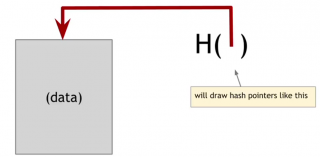
\includegraphics[scale=0.8]{hash_pointer}
\caption{Hash pointer}
\end{figure}

Iz definicije se vidi da hash pointer nije ništa revolucionarno novo već samo pametna kombinacija alata koji su postojali i prije. Primjetimo da se sami podaci na koje pokazuje hash pointer ne moraju kriptirati, što je ogromna prednost jer nama sama hash vrijednost podataka garantira da nije bilo promjena (naravno uz uvjet da hash vrijednost bude sigurno spremljena). Također hash pointeri su toliko jednostavna struktura da ju možemo koristiti u implementaciji već poznatih većih struktura podataka lista, binarno stablo i sl.

\begin{figure}[!]
\centering
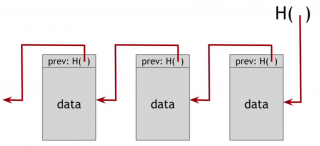
\includegraphics[scale=0.9]{blockchain}
\caption{Blockchain}
\label{fig:blockchain}
\end{figure}

Blockchain je vezana lista čije su veze hash pointeri. Očita razlika od obične vezane liste koja prozilazi iz toga da je veza hash pointer jest u tome da svaki blok sadrži informacije ne samo o sebi, već i o prijašnjem bloku. 

Kombinacija transparentnosti i nepromjenjivosti, koja je spomenuta u definiciji \ref{def:block}, postignuta je pametnim korištenjem hash pointera. Da objasnimo zašto je to tako trebamo se zapitati što bi se desilo kada bi napadač htio promjeniti neki podatak napisan na blockchinu. Recimo da se taj podatak nalazi u bloku indexa $k$. Ako napadač promjeni sadržaj tog bloka, tada će se razlikovati i njegova hash vrijednost, a upravo ta hash vrijednost se nalazi u bloku $k+1$. Što znači da će napadač promjeniti i sadžaj bloka $k+1$, tj. promjeniti i njegovu hash vrijednost itd. Dakle vidimo ako napadač želi sakriti svoju jednu promjenu u podacima trebat će mjenjati sve blokove koji dolaze nakon bloka u kojem je nastala promjena. Znači pod uvjetom da \textbf{sigurno spremimo hash pointer samo zadnjega bloka} možemo garantirati za ispravnost sadržaja cijelog blockchaina. No u prethodnoj definiciji blockchain je naveden kao distribuirano spremište podataka (dakle čuva se na mreži), pa u takvoj situaciji nije praktično da svaki čvor mreže na kojoj se nalazi blockchain mora spremati hash pointer zadnjeg bloka jer mreža je asinkrona i lanac nije svugdje iste duljine. U tom slučaju ako dizajniramo komunikacijski protokol gdje svaki čvor čuva cijeli lanac i pri međusobnoj komunikaciji uzima se najdulji lanac kao ispravan, tada uz uvjet da je \textbf{50\% mreže iskreno} možemo garantirati sigurnost blockchaina. Također zbog svojstva distribuiranosti i lakšeg transaporta po mreži valjalo bi i ograničiti veličinu bloka. No danas, memorija nije skup resurs, tako da u teoriji u pojedine blokove možemo spremati podatke proizvoljne veličine.

\section{Bitcoin}

Danas većina ljudi pod pojmom Bitcoin na digitalni novac pomoću kojeg se obavljaju transakcije. No Bitcoin je cijela zasebna platna mreža u kojoj digitalni token služi kao sredstvo za izvršavanje transakcija. Na toj mreži se zapravo nalazi samo jedan blockchain koji sadrži popis svih transakcija koje su se ikad desile na mreži. U tehničkom smislu ta mreža je zapravo jedna \textit{peer-to-peer} mreža, što znači da nema centralne jedinice koje dijeli blockchain već svaki čvor mreže mora imati svoju kopiju blockchaina. On ju redovito održava i osvježuje u komunikaciji sa susjednim čvorovima. Pojedini čvor ne zna tko su mu susjedi i svaku informaciju koju dobije kompletno provjerava za sebe. U slučaju da od susjeda dobije lance različitog sadržaja, protokol pretpostavlja da je lanac najveće duljine točan. Ključna stvar koja se postiže ovakvom definicijom je decentralizacija. Na mreži žive korisnici koji komuniciraju između sebe jedino pomoću transakcija (dakle jedino što mogu jest izmjenjivati tokene) koje se konstantno zapisiju na blockchain. 

\begin{napomena}
Uočimo bitnu razliku između korisnika i čvorova. Čvor je fizičko računalo koje održava Bitcoin mrežu aktivnom, dok je korisnik zapravo korisnik te mreže koji obavlja transakcije. Ako imamo skup čvorova $ČVOR$ i skup korisnika $KORISNIK$ tada vrijedi relacija $ČVOR \subsetneqq KORISNIK$.
\end{napomena}

Recimo da korisnik Alice napravi transakciju s kojom želi poslati 3 tokena (tj. Bitcoina) korisniku Bob. Ta transakcija koju Alice zatraži prvo ide u skup svih neobrađenih transakcija. Taj skup sadrži sve transakcije koje čekaju da ih čvorovi izvrše i zapišu na blockchain. Čvor prvo uzme $n \in \mathbb{N}$ transakcija i provjerava svaku od njih. Pod pojmom provjerava mislimo prolazak kroz sve prethodne transakcije uključenih korisnika i odlučivanje da li je tražena transakcija valjana, tj. da li korisnik koji šalje tokene, zapravo ima broj tokena koji želi poslati. 

\begin{napomena}
Primjetimo da je ova provjera svih prethodnih transakcija nužan uvjet jer nigdje na blockchainu ne postoji zapis koliko pojedini korisnik ima tokena, već samo njegove transakcije. Također primjetimo da se nema nikakve provjere primatelja, dakle ako je napisana kriva adresa primatelja poslani tokeni će biti izgubljeni.
\end{napomena}

Ako su sve transakcije valjane tada se taj blok emitira na mrežu i on će postati idući blok u blockchainu. Da bi postao dio lanca treba nam njegov hash pointer tako da sada svi čvorovi skupa pokušavaju izračunati hash vrijednost bloka. U račun te hash vrijednosti ne ulazi samo sadržaj bloka već i salt, tj. proizvoljan broj koji ubacujemo jer nam treba hash vrijednost takva da vrijedi:

\begin{equation}
\label{eq:hash}
    H(salt\ |\ kompletan\ sadržaj\ bloka) \leq granica
\end{equation}

\begin{definicija}
Granica je broj jedinstven za cijelu mrežu i kojeg sama mreža računa ispočetka svakih sat vremena ovisno o procesorskoj snazi mreže, točnije koliko hash vrijednosti mogu svi čvorovi na mreži izračunati u jednoj sekundi.
\end{definicija}


Izračunati novu hash vrijednost jedino se može \textit{brute force algoritmom}, dakle nasumičnim pogađanjem raznih vrijednosti salta želi se dobiti hash vrijednost koja je manja od granice. Ta metoda je izrazito procesorski zahtjevna i zbog toga nije  pogodno koristiti kućno računalo kao čvor na Bitcoin mreži. Kao poticaj da ipak ljudi imaju čvorove, prvi koji izračuna hash vrijednost za nagradu dobije  tokene (Bitcoine). Kada se dobije hash vrijednost tada taj blok postaje idući u blockchainu. Proces generacije novog bloka i ujedno stvaranja novih Bitcoina se naziva \textbf{rudarenje}.

\begin{figure}[H]
\centering
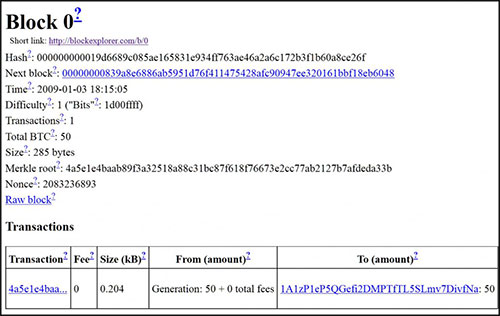
\includegraphics[scale=0.5]{genisis_block}
\caption{ \textit{genesis blok} - prvi blok u Bitcoin blockchainu.}
\end{figure}

Ovo je sve što ćemo općenito reći o Bitcoinu i jedino ćemo detaljnije predstaviti 3 stvari koje će mi kasnije koristiti u ovom radu: identifikacija korisnika na mreži, transakcije i transakcijske skripte. Prvo ćemo dati rješenje \textbf{decentraliziranog sustava identifikacije} korisnika na mreži. U prethodnom dijelu smo dali definiciju digitalnog potpisa koji služi za autorizaciju u digitalnom svijetu, no on sam od sebe nije dovoljan za idenitifikaciju jer bi u tom slučaju također trebali imati centralnu jedinicu koja će upravljati ključevima. Bitcoin problem identifikacije rješava zanimljivim trikom da se uzima javni ključ iz sheme digitalnog potpisa kao identitet korisnika, točnije za to koristi već spomenuti digitalni potpis ECDSA. Posljedica uzimanja javnog ključa kao digitalnog identiteta jest da fizička osoba koja kontrolira korisnika mreže (dakle posjeduje privatni ključ) nije nikako vezana za njega, već si može generirati novi par ključeva i stvoriti novoga korisnika kada god poželi. Također već smo rekli da u ECDSA ključevi su proizvoljni 256-bitni niz nula i jedinica, dakle nema gotovo nikakve sanše da se korisnika mreže poveže sa fizičkom osobom tako da imamo i prilično veliku razinu anonimnosti na mreži.

Sada kada imamo sustav identifikacije možemo opisati kako izgleda transakcija između korisnika na Bitcoin mreži. Transakcija je običan JSON objekt koji se vidi na slici \ref{fig:transakcija} koji se sastoji od 3 glavna dijela:
\begin{enumerate}
    \item \textit{metapodaci} - jedini bitan dio metapodataka nam je hash cijele transakcije, koji služi kao ID transakcije
    \item\textit{ulazne transakcije} - blockchain ne sadrži informaciju koliko pojedini korisnik sadrži tokena, već se svaka transakcija referencira na neku prijašnju u kojoj je taj korisnik sudjelovao
    \item \textit{izlazni podaci} - izlazna vrijednost transakcije i \textbf{transakcijska skripta}
\end{enumerate}

\begin{figure}[H]
\centering
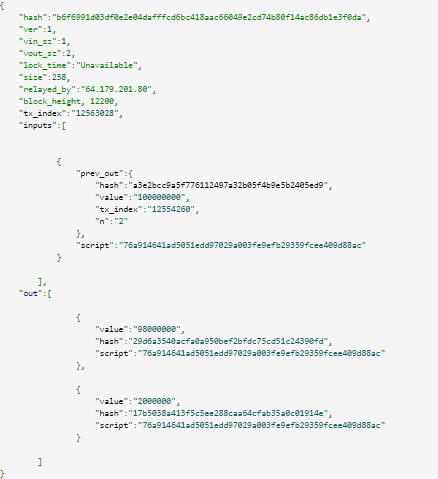
\includegraphics[scale=0.73]{transakcija}
\caption{Bitcoin transakcija}
\label{fig:transakcija}
\end{figure}

Nama najzanimljiviji dio transakcije je transakcijska skripta. Pod tim pojmom mislimo na kodirani računalni program pisan u jeziku Script. Taj program se izvršava prilikom prvog procesiranja transakcije i zapisivanja na blockchain. Kod toga programa sam se generira i nije programibilan. 

Script\cite{script} je programski jezik napravljen specifično za Bitcoin. Izvršava se na stogu, vrlo je jednostavan (ima mjesta za samo 256 naredbi, tj svaka naredba je kodirana u 2 broja u heksadecimalnom zapisu), nije Turing-kompletan i nema petlji.

\chapter{Ethereum}

Dok je Bitcoin zamišljen za specifičnu svrhu decentraliziranog izvršavanja financijskih transakcija, 2013. godine Vitalik Buterin je u svoj radu\cite{eth_paper} predstavio svoju ideju za novu generaciju blockchaina nazvanu Ethereum, čiji je cilj izvršavanje proizvoljnih programa, tj. pametnih ugovora. U ovom poglavlju ćemo predstaviti Ethereum i pokušati objasniti napredak u odnosu na svoje prethodnike.

\section{Općenito}

S obzirom da mnogo ljudi dolazi do Ethereuma sa nekim prijašnjim iskustvima i znanjem o Bitcoinu, odmah na početku ćemo naglasiti razlike s obzirom da svoje prethodnike, pa po \cite{ethbook}:

\begin{definicija}
Ethereum je \textbf{globalno distribuirana računalna mreža} koja izvršava programe zvane pametni ugovori. Mreža koristi blockchain za sinkronizaciju i spremanje promjena stanja mreže, a valutu zvanu \textbf{ether} za mjerenje i ograničavanje resursa mreže.
\end{definicija}

Vidimo odmah da je namjera ove definicije predstaljanje Ethereum kao mreže koja će biti poslužitelj pametnim ugovorima, tj. decentralizirana platforma za aplikacije, a digitalna valuta je samo sredstvo koje se koristi da bi mreža ispravno funkcionirala. Zbog toga bi se moglo zaključiti da građa Ethereuma potpuno drukčija od ostalih kriptovaluta no iznenađujuće, to uopće nije slučaj.

I dalje je to u srcu blockchain koji kao i prije sadrži popis svih transakcije koje su se ikada desile, no stvar zbog koje je Ethereum bitno napredniji od svih svojih prethodnika jest funkcionalnost tih samih transakcija. Bitcoinove transakcije su prilično jednosmjerne, jedino mogu izmjenjivati tokene između korisnika (uz male varijacije). U Ethereumove transakcije moguće je poslati proizvoljan program sa prilagođenom logikom koji se nakon toga izvršava na mreži. Dakle ako zamislimo da je Bitcoin blockchain koji prati stanje koliko koji korisnik ima tokena, tada Ethereum možemo zamisliti kao blockchain koji prati stanje podataka proizvoljnog oblika.

Taj računalni program koji šaljemo transakcijom se naziva \textbf{pametni ugovor}, a cijeli proces nam omogućuje \textbf{Ethereum Virutal Machine} u kojem se izvršava kod programa. Ethereum Virtual Machine (kao i svaki virtual machine) je sloj apstrakcije između koda koji se izvršava i fizičkog računala koje izvšava kod, tj. sloj koji programski kod pisan u high level jezicima preslikava u low level\textbf{bytecode} (primjer bytecoda \ref{eq:bytecode}).

\begin{napomena}
low leveljezik je zapravo niz nula i jedinica razumljivih računalu koje ih izvodi, ali nama ljudima ne znači previše. Suprotno od toga postoje high level jezici koji imaju snažnu ogradu od apstrakcije računala koje izvodi program. Dakle svi programski jezici koje mi ljudi pišemo su primjeri high level jezika.
\end{napomena}

\begin{dmath}
0x608060405234801561001057600080fd5b5061018e806100206000396000f3\\fe608060405260043610610041576000357c0100000000000000000000000000\\000000000000000000000000000000900463ffffffff1680631e2aea0614610\\046575b600080fd5b34801561005257600080fd5b50610109600480360360208\\1101561006957600080fd5b8101908080359060200190640100...
\label{eq:bytecode}
\end{dmath}


\section{Korisnici}

Princip identifikacije korisnika na mreži je također potpuno isti kao i prije, koristi se javni ključ iz sheme digitalnog potpisa ECDSA za identifikaciju uz jednu veliku razliku. Na Ethereumu postoje dvije vrste korisnika: 
\begin{enumerate}
    \item \textit{user korisnici}
    \item \textit{contract korisnici}
\end{enumerate}

\begin{figure}[H]
\centering
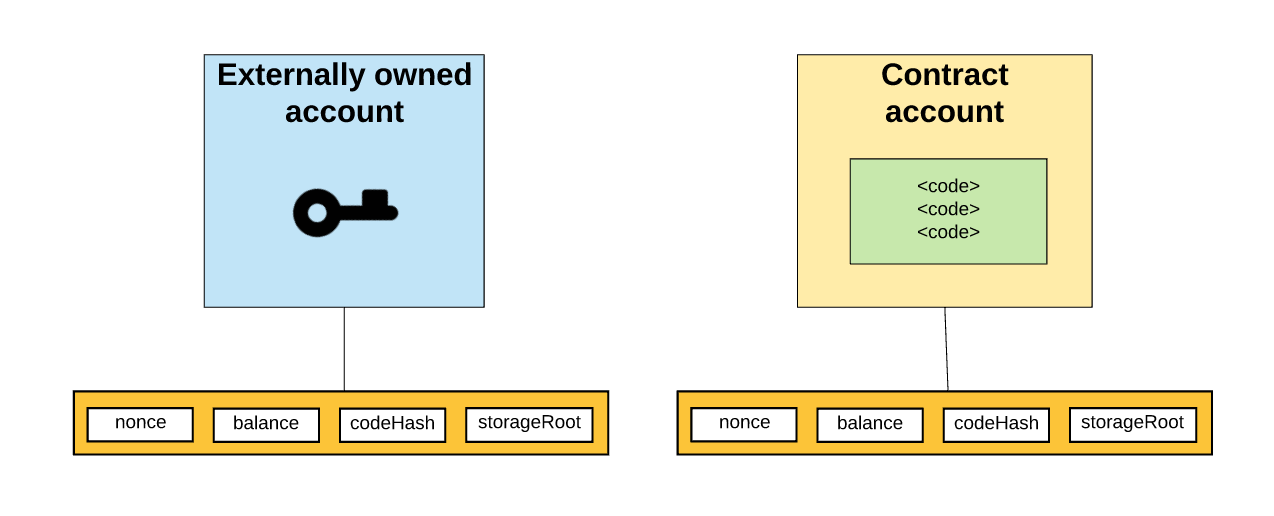
\includegraphics[scale=0.32]{ethaccounts}
\caption{Ethereum korisnici}
\label{fig:ethaccounts}
\end{figure}

Kod Bitcoina je ponašanje svakog korisnika je bilo kontrolirano od strane neke fizičke osobe koja posjeduje privatni ključ tog korisnika, tj. postojali su samo user korisnici. Ovdje postoji i drugi tip korisnika, a to su adrese na kojima se nalaze pametni ugovori. Kao što se vidi sa slike \ref{fig:ethaccounts} izvana su ti korisnici jednaki (oba sadrže ether, oba mogu slati i primati transakcije), jedina razlika jest što ponašanje korisnika na čijoj je adresi pametni ugovor, definirano pomoću koda koji se nalazi u njemu.

Kao i kod Bitcoina svaki čvor na mreži izvršava sve poslane transakcije i zapisuje stanje cijele mreže. S obzirom da bilo koji user korisnik može napisati pametni ugovor i poslati ga na mrežu, a nisu svi user korisnici pouzdani, može doći do pretjeranog iskorištavanja resursa čvorova na mreži, npr. u slučaju da pametni ugovor u sebi ima zapisan \textbf{halting problem} i taj ugovor bude poslan na mrežu, cijela mreža nebi nikad procesirala nijednu drugu transakciju. Zbog toga je uveden sustav naplate naknade za izvršvanje svakog koraka u kodu transakcije i taj sustav ćemo promotriti u idućem odjeljku.

\section{Gas}

Na mreži Ethereum postoje dva tokena: \textbf{ether} i \textbf{gas}. Ether ne trebamo pretjerano objašnjavati jer je to digitalna valuta koja se nalazi na Ethereumu i ima fizičku protuvrijednost (na ether zapravo većina ljudi misli kada se kada spomene Ethereum), dok je gas cijena izvršavanja transakcija i rada mreže. Vrijednost gasa se postavlja od strane korisnika u etheru pri slanju transakcije te taj broj nije fiksan.

\begin{tcolorbox}
Već u samom imenu gas vidimo analogiju sa stvarnim svijetom. Možemo zamisliti gas kao benzin, novac kao ether, a auto kao cijelu Ethereum mrežu. Novcem kupujemo benzin koji je neophodan da bi auto radio. Isto tako ovdje etherom kupujemo gas koji je neophodan da bi Ethereum mreža radila, tj. procesirala transakcije i zapisivala ih na blockchain.
\end{tcolorbox}

Uz svaku transakciju koja se šalje na mrežu, korisnik koji ju šalje treba postaviti dvije vrijednosti:

\begin{itemize}
    \item \textbf{gas limit} - maksimalna količina gas-a koju transakcija smije potrošiti na svoje izvršavanje
    \item \textbf{cijena gasa} - vrijednost 1 gasa u etheru
\end{itemize}

Dakle dobivamo da je ukupna maksimalna vrijednost transakcije:
\begin{equation*}
    maksimalna\ vrijednost\ transakcije = gas\ limit \times cijena\ gasa
\end{equation*}

Kažemo maksimalna vrijednost transakcije jer ne znamo za sve transakcije točan iznos koji ćemo potrošiti s obzirom da možemo slati proizvoljan kod koji može ovisiti o argumentima koje pošaljemo. U slučaju da nije potrošen puni iznos koji smo naveli tada se ostatak vraća pošiljatelju, ali u slučaju da transakcija nije prošla, iz bilo kojeg razloga, potrošeni gas (tj. ether) se gubi zauvijek. Iznos ethera za koji je potrošeno gasa u transakciji će dobiti čvor koji prvi procesira transakciju i zapiše ju na blockchain. Primjetimo da mi sami određujemo koliko ćemo platiti jedinicu gasa, tj. maksimalnu ukupnu vrijednost koliko smo spremni platiti transakciju. S obzirom da čvorovi koji procesiraju transakcije sami odbiru koje će transakcije procesirati, vrlo je vjerojatno što veći iznos stavimo za cijenu gasa i samim time povećamo joj vrijednost, da će nam transakcija brže biti izvršena.

Također primjetimo da cijelo vrijeme govorimo transakcije i iako pod tim mislimo zapravo kod koji se izvršava, iako je izraz transakcija ispravan jer kao i kod Bitcoina jedino pomoću njih se mjenja stanje mreže i pokreću programi.

Sada kada imamo objašnjenu naplatu izvršavanja transakcija, promotrit ćemo primjere iz stvarnog svijeta koliko je skupo održavati aplikaciju na Ethereumu. Na slici \ref{fig:ethunits} se nalazi tablica pretvaranja jedinica ethera.

Primjeri cijene gasa u "standardnim" uvjetima (nemoguće je točno definirati standardne uvjete jer se broj čvorova konstantno mjenja, a s time i procesorska moć mreže): 
\begin{itemize}
    \item 40 GWEI - gotovo je sigurno da će transakcija biti zapisana u idući blok (vrijeme potrebno za 1 blok je u prosjeku 13 sekundi)
    \item 20 GWEI - prosjek, gotovo sigurno će transakcija biti zapisana u idućih par blokova
    \item 2 GWEI - gotovo sigurno će transakcija biti procesirana u idućih par minuta
\end{itemize}

\begin{figure}[H]
\centering
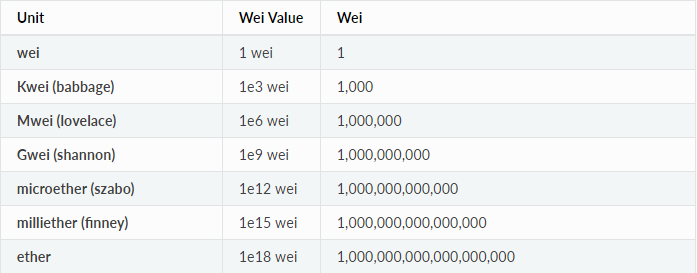
\includegraphics[scale=0.55]{ether_units}
\caption{Pretvorba jedinica ethera}
\label{fig:ethunits}
\end{figure}

\newpage

Kao što smo prije napomenuli, svaki program se pomoću Ethereum Virtual Machina kompajlira u bytecode. Bytecode je zapravo kodiran jedan \textbf{assembly} program. Assembly program je niz jednostavnih opracija zvanih \textbf{optkodovi}. Optkodovi se izvršavaju na stogu i ovisno o kompleksnosti pojedinih operacija imaju različitu cijenu izvođenja izraženu u gasu. 

\begin{napomena}
Naziv assembly nema veze sa istoimenim programskim jezikom, iako vidimo sličnost zbog jednostavnosti kao i jednakosti nekih operacija.
\end{napomena}

\begin{center}
\begin{tabular}{c|c|c}
     Optkod & Cijena (gas) & Opis optkoda \\
     \hline
     ADD & 3 & zbroj 2 broja \\ \hline
     MUL & 5 & množenje 2 broja \\ \hline
     SHA256 & 60 & računanje SHA-256 hash funkcije \\ \hline
     BALANCE & 700 & dohvaćanje količine ethera koju korisnik ima na računu \\ \hline
     SSTORE & 20000 & spremanje riječi u memoriju ugovora \\ \hline
     CREATE & 32000 & kreiranje novog korisnika sa zadanom adresom (najskuplji optkod)
    
\end{tabular}
\end{center}

Na prethodnoj tablici vidimo cijene izvršavanja pojedinih optkodova. Kao što vidimo nema jedinstvene operacije za prijenos ethera sa adrese jednog korisnika na drugi, već je to skup kodova. Ovdje nećemo ulaziti u detalje koji su to kodovi, ali prema \cite{wood2014ethereum} ukupna vrijednost tih kodova je 21000 gasa. Računom dobijemo:

\begin{itemize}
    \item 30 GWEI - cijena gasa tako da transakcija bude izvršena unutar 1 minute (u prosjeku)
    \item 171,56 USD - trenutna cijena 1 ethera
    \item 21000 gasa - prijenos ethera s jedne adrese na drugu
\end{itemize}

\begin{minipage}{\linewidth}
\begin{equation*}
    30\ GWEI = 0.00000003\ ETH
\end{equation*}
\begin{equation*}
    21 000\ gas \times 0.00000003\ ETH = 0.00063\ ETH
\end{equation*}
\begin{equation*}
    0.00063\ ETH \times 171.56\ USD = 0.11\ USD = 0.72\ HRK 
\end{equation*}
\hspace{0.5cm}
\end{minipage}

Dakle uz naknadu od 0.72 kn se može prenijeti proizvoljna količina ethera u roku jedne minute na adresu na koju se može pristupiti bilo gdje u svijetu što je veliki napredak u usporedbi korištenja banaka. No s obzirom da su tema ovoga rada pametni ugovori promotrimo sada primjer ove jednostavne funkcije ugovora.  

\begin{minipage}{\linewidth}
\begin{lstlisting}[caption = Primjer 1, language=solidity, label={lst:suma}]
function sumArray(uint[] memory arrayToSum) pure returns (uint _sum) {
    _sum = 0;
    for (uint i = 0; i < arrayToSum.length; i++) {
        _sum += arrayToSum[i];
    }
}
\end{lstlisting}
\end{minipage}

U primjeru \ref{lst:suma} vidimo funkciju koja sadrži deklaraciju varijable te for petlju koja prolazi poljem brojeva i zbraja njegove članove. Cijena izvršavanja te funkcije očito ovisi o duljini toga polja.

\begin{lstlisting}[language={[x86masm]Assembler}, caption=Assembly program od funkcije iz primjera \ref{lst:suma}]
tag 52 JUMPDEST, PUSH 0, DUP1, SWAP1, POP, PUSH 0, DUP1, SWAP1, POP, tag 53 JUMPDEST, DUP3, MLOAD, DUP2, LT, ISZERO, PUSH [tag] 54, JUMPI, DUP3, DUP2, DUP2, MLOAD, DUP2, LT, PUSH [tag] 56, JUMPI, INVALID, tag 56 JUMPDEST, PUSH 20, MUL, PUSH 20, ADD, PUSH 20, ADD, ADD, MLOAD, DUP3, ADD, SWAP2, POP, DUP1, DUP1, PUSH 1, ADD, SWAP2, POP, POP, PUSH [tag] 53, JUMP, tag 54 JUMPDEST, POP, SWAP2, SWAP1, POP, JUMP [out]   
\end{lstlisting}

Dakle ako imamo polja duljine: 

\begin{itemize}
    \item 1 - cijena je samo 170 gasa sto je zanemariva stvarna protuvrijednost
    \item 100 - cijena je $\approx$ 17000 gasa, a ako postavimo cijenu gasa na 30 GWEI (potvrda transakcije unutar 1 minute), dolazimo do cijene od 17000 gas $\times$ 30 GWEI = 510000 GWEI = 0.00051 ETH = 0.08 USD = 0.58 HRK što je zapravo prilično velika cijena za dobiti sumu polja sa 100 brojeva
\end{itemize}

Vidimo da iako imamo prilično jednostavnu operaciju iznos može vrlo brzo narasti do granice isplativosti izvođenja, zato pri programiranju pametnih ugovora treba biti posebno oprezan što ćemo i vidjeti u idućem poglavlju.

\chapter{Pametni ugovori}

U prvom poglavlju smo krenuli od najosnovnije kriptografije i blockchaina, kasnije ukratko predstavili Bitcoin te na kraju elemente Ethereuma. U ovom poglavlju ćemo napokon objasniti kako funkcionira sam pametni ugovor, njegove mogućnosti i na kraju pogledati sigurnost.

\section{EVM \& Solidity}

Kao što smo rekli pametni ugovor se izvodi u Ethereum Virtual Machinu (skraćeno EVM). EVM je "stack-based" virtual machine, tj. sve operacije se izvršavaju na stogu. Kompletno je izoliran od računala na kojem se nalazi (što znači da nema pristup filesystemu, mreži i sl.), ima neograničenu memoriju, ali što se više memorije koristi to više košta gasa, dakle granice u EVMa nisu statične već ekonomske. Da bi dobili bytecode koji EVM zna čitati, trebamo imati neki high level jezik koji je čitljiv nama ljudima, a da može se prevesti u njega. Primjera takvih jezika je mnogo: Vyper, Bamboo, LLL, ali najpopularniji među njima je \textbf{Solidity}. Dizjniran je upravo od tima programera koji su implementirali Ethereum mrežu i pravljen specifično za pisanje pametnih ugovora, Solidity je objektno orijentirani \textbf{Turing potpun} jezik vrlo sličan Javascriptu.

\begin{napomena}
Turing potpunost znači da se može izvršiti program proizvoljne kompleksnosti uz neograničenu memoriju.
\end{napomena}

Upravo u toj Turing potpunosti se vidi velik napredak u odnosu na Bitcoin, jer ako se prisjetimo Bitcoinova transakcijska skripta može samo izvršiti razmjenu tokena između korisnika. Također valja napomenuti da nemaju svi gore navedeni jezici iste karakteristike iako se kompajliraju u isti bytecode, npr. Vyper nije uopće Turing potpun, ali zbog tih smanjenih mogućnosti je puno sigurniji od Solidityja.

\section{Izvršavanje koda}

Kao na Bitcoinu, svaka promjena stanja na Ethereumu zahtjeva slanje neke transakcije. Pri svakom slanju moramo specificirati adresu primatelja i sadržaj transakcije, što je prilično očekivano. Rekli smo da na Ethereumu postoje dvije vrste korisnika: user i contract korisnici. Ako smo specificirali da poruku prima user korisnik tada sve što ta transakcija radi je prebacuje ether, no ako smo specificirali contract korisnika tada aktiviramo pametni ugovor i počinje se izvršavati kod. Pametni ugovor \textbf{nema stanje} i slanjem transakcija jedino ga je moguće aktivirati (ovaj dio je naglašen jer to znači da je nemoguće imati funkcije koje se same pokreću, npr. periodičke funkcije ili jobovi). Kod pametnih ugovora može:

\begin{itemize}
    \item Slati ether na željene adrese
    \item Čitati/pisati iz svoje memorije
    \item Pozivati izvršavanja drugih pametnih ugovora
\end{itemize}

Znamo da se ugovor piše u nekom high level jeziku koji se onda kompajlira u bytecode. Taj bytecode se zatim objavljuje na Ethereum mrežu tako da se pošalje transakcijom (kao transakcijska skripta) na adresu koja još nije iskorištena i na mreži se pokreće ponovnim slanjem nove transakcije na tu adresu. No kako pozvati točno određenu funkciju na ugovoru? Pri kompajliranju pametnih ugovora dobijemo mnogo informacija: bytecode,  \textbf{Application Binary Interface} (skraćeno ABI), assembly, procjene gasa, potpis i još dosta ovdje nebitnih informacija.

\begin{definicija}
ABI je interface između dva programska modula, od kojih jedan je često na nivou strojnog koda (niz nula i jedinica), a drugi program kojeg pokreće čovjek. 
\end{definicija}

U kontekstu Ethereuma, ABI je lista svih \textbf{potpisa funkcija} koje se nalaze u pametnom ugovoru, a mogu piti pozvane izvana (primjetimo da privatne funkcije se ne nalaze na ABI-ju). Na primjeru \ref{fig:abi} vidimo potpis funkcije iz primjera \ref{lst:suma}. Odmah primjećujemo da je to zapravo jedan običan JSON objekt (kao i sve u Ethereumu). Kodiranjem nekih vrijednosti tog JSON objekta, zajedno sa našim argumentima i slanjem dobivenog koda transakcijom pozivamo funkcije pametnog ugovora, a za detalje kodiranja promotrimo sljedeći primjer:

\begin{figure}[H]
\centering
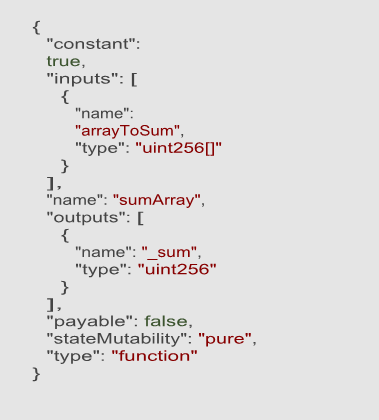
\includegraphics[scale=0.8]{abi}
\label{fig:abi}
\end{figure}

Kao što smo rekli na prethodnoj slici je potpis funkcije $sumArray$ iz primjera \ref{lst:suma} i ako želimo pozvati tu funkciju $sumArray([164, 46])$ tada bi poslali ukupno 36 bytova koji izgledaju: 


\begin{dmath}
\label{eq:sumabi}
    0x1e2aea06a40000000000000000000000000000000000000000000\\00000000000000000002e000000000000000000000000000000000\\00000000000000000000000000000
\end{dmath}

Taj kod nam ne znači previše, ali ako razdvojimo na svoje djelove dobijemo: 

\begin{itemize}
    \item Prvih 4 bytea je ID funkcije. ID se dobije tako da se uzme početak hash vrijednosti potpisa funkcije, tj. u ovom slučaju primjeni Keccak256 (SHA256) hash funkcija na $arraySum(uint256[])$
    \begin{equation*}
        h(arraySum(uint256[])) = \textbf{1e2aea06}47440989b12156a7890618f416...
    \end{equation*}
    \item Ostatak su argumenti funkcije. Uvijek je to zapravo njihova hex vrijednost proširena da ima veličinu 32 byta. S obzirom da je ovdje polje brojeva u pitanju proširenje s nulama će doći s desne strane hex vrijednosti.
    \begin{equation*}
        paddedHex(164) = 0xa400000000000000000000000000000000000000...
    \end{equation*}
        \begin{equation*}
        paddedHex(46) = 0x2e000000000000000000000000000000000000000...
    \end{equation*}
\end{itemize}

Algoritam takvog kodiranja se zove \textbf{Recursive Length Prefix} i kompleksniji primjeri se nalaze na \cite{rlp}.

Još samo za kraj ćemo napraviti provjeru da nismo pogriješili u algoritmu. Naime pametni ugovor čiji se bytecode nalazi u primjeru \ref{eq:bytecode} sadrži funkciju $sumArray$ i što znači da taj bytecode mora imati ID te funkcije $1e2aea06$, a to je istina jer:

\begin{dmath}
0x608060405234801561001057600080fd5b5061018e806100206000396000f3\\fe608060405260043610610041576000357c0100000000000000000000000000\\000000000000000000000000000000900463ffffffff168063\textcolor[rgb]{1,0,0}{1e2aea06}14610\\046575b600080fd5b34801561005257600080fd5b50610109600480360360208\\1101561006957600080fd5b8101908080359060200190640100...
\label{eq:bytecode_red}
\end{dmath}

\section{Sigurnost}

U ovom trenutku postoji više od 1 000 000 pametnih ugovora na Ethereumu koji skupa posjeduju preko 100 000 000 ethera u sebi. Zbog takovg kapitala posebno su zanimljivi hakerima. Pametni ugovori su nova tehnologija i već kao takva daju izazove jer nema standardiziranog principa razvoja. Također, objavljeni su na blockachainu i jednom kada se pošalju na mrežu ne mogu se mjenjati i nadograđivati tako da svaka greška ostavlja trajne posljedice. Primjer jedne takve greške je \textbf{DAO hack} (dio koda koji je hakiran je na primjeru \ref{lst:hack}) koji se dogodio 2016. godine u kojem je ukradeno 50 000 000\$ i zbog kojega se Ethereum blockchain morao razdvojiti na dva lanca. Napravljen je novi lanac čije je stanje jednako onome prije hacka (dakle vraćene su sve transakcije) i danas je to Ethereum, dok je lanac na kojem se dogodio hack nastavio živjeti i danas se on zove Ethereum Classic.

\begin{minipage}{\linewidth}
\begin{lstlisting}[caption = Ukratko: DAO je jedna od drugih valuta na Ethereumu nastala slanjem pametnog ugovora i njena protuvrijednost je u etheru. Funkcija \lstinline{withdraw} jednostavno povlači sredstva koje korisnik ima na DAO pametnom ugovoru. No što ako damo hrpu zahtjeva odjednom? Tada se sredstva konstantno prebacuju na račun korisnika no na pametnom ugovoru se nije uspio smanjiti broj jer nije postojao nikakav mehanizam zaštite., language=solidity, label={lst:hack}]
function withdraw(uint _amount) public {
  if(balances[msg.sender] >= _amount) {
    if(!msg.sender.call.value(_amount)()) { 
        throw;
    }
    balances[msg.sender] -= _amount;
  }
}
\end{lstlisting}
\end{minipage}

\newpage

Još jedno ograničenje koje je bitno jest naplata izvođenja koda, dakle funkcionalnost je "bitnija" od sigurnosti. To izvođenje znamo da se vrši iz bytecoda na koji mi imamo jedini utjecaj preko high level jezika u kojima pišemo. Dakle sigurnost pametnih ugovora zapravo proizlazi iz sigurnosti samog high level jezika u kojem su napisani.

Solidity je Turing potpun jezik rađen po uzoru na Javascript, a Javascript nije poznat kao siguran jezik. Dakle i Solidity ima standardne probleme kao što su overflow i underflow. No Solidity strašno brzo napreduje (službeno po Githubu 315 ljudi ga razvija i od prosinca 2015. je doživio čak 59 izdanja), popravlja probleme svakim novim izdanjem, ali i dalje postoje sumnje u Solidity kao pravi jezik za pametne ugovore. Upravo se mnogo ljudi zalažu za neke Turing nepotpune jezike poput Vypera koji mogu većinu operacija izvesti kao i Solidity no mnogo su sigurniji. Vyper je također objektno orijentirani jezik vrlo sličan Pythonu. Njegove ključne karakteristike zbog čega je postao popularan u jako kratkom roku (prvo izdanje Vyper je doživio u ožujku 2018. godine) su: sigurnost, jednostavnost jezika i čitljivost. 

Još bi samo htio na kraju reći malo o sigurnosti s legalne strane. Naime trenutno nigdje ne postoji niti jedan članak zakona kojim bi se pametni ugovori predstavljali kao zakonski ugovor (ili barem nešto slično tome) što je prilično interesantna činjenica s obzirom da ima toliki ogroman kapital pohranjen u sebi.
    
\chapter{Primjer: Crypto Roulette}

Sa prethodnim poglavljem samo zaključili svu potrebnu teoriju za razumjevanje funkcionalnosti pametnih ugovora. No trenutno sva ta teorija je nekako u svom "ekosustavu" i nije potpuno jasno kako ju uklopiti u današnji svakodnevni život, s time dolazimo do svijeta \textbf{decentraliziranih aplikacija} koji se popularno naziva \textbf{Web 3.0}.

\section{Decentralizirane aplikacije}

Kao što smo rekli u definiciji \ref{def:dapp}, decentralizirana aplikacija je open source aplikacija koja se izvršava na nekoj blockchain mreži. Svaka aplikacija se sastoji od frontend, ono što vidimo, te backend dijela, sama logika aplikacije (naravno takva podjela je jako pojednostavljeno stanje). backend dio uobičajenih aplikacija se izvršava na nekom centralnom serveru, dok kod decentraliziranih aplikacija na nekoj blockchain mreži. S obzirom da su tema ovoga rada pametni ugovori, u našem slučaju backend dio naše decentralizirane aplikacije jedan je sustav pametnih ugovora, koji se izvršavaju na Ethereumu. 

\begin{napomena}
U prethodnoj definiciji smo naveli "sustav pametnih ugovora", naime aplikacija može sastojati od skupa ugovora koji komuniciraju međusobno pomoću transakcija.
\end{napomena}

\begin{figure}[h]
\centering
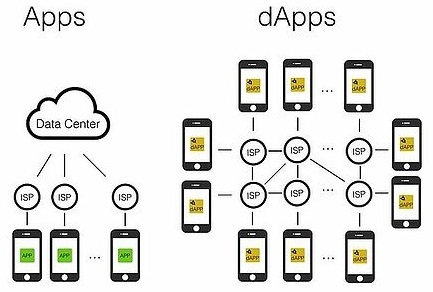
\includegraphics[scale=0.7]{AppsVSdApps}
\caption{Apps VS. dApps}
\label{fig:appvsdapp}
\end{figure}

Na slici \ref{fig:appvsdapp} vidimo glavnu razliku između decentraliziranih i uobičajenih aplikacija, one imaju centralnu bazu podataka koja pruža samo nužne podatke korisniku, za razliku od decentralizirane aplikacije gdje se svi podaci nalaze na Ethereumu (točnije pametnom ugovoru), dakle svaki korisnik u bilo kojem trenutku ima dostupnu kompletnu bazu podataka aplikacije. Ta razlika je posljedica upravo činjenice da se decentralizirana aplikacija nalazi na blockchain mreži koja je u potpunosti transparentna. Iz prethodnih poglavlja znamo da svaki korisnik može sam mjenjati zapise na blockchainu ta baza je ujedno i decentralizirana (ako nije u pametnom ugovoru zadano suprotno). Transparentnost i decentraliziranost su zasigurno pozitivna promjena od uobičajenih aplikacija, no te promjene dolaze sa cijenom. Svako izvršavanje koda i spremanje podataka na Ethereumu košta neki iznos ethera koji se s količinom spremljenih podataka povećava. Dakle pri izradi decentralizirane aplikacije treba biti vrlo oprezan sa arhitekturom logike aplikacije. Neke aplikacije čak koriste tzv. "off-chain izvore" (izvore koji se ne nalaze na blockchainu i ne koriste njegove resurse) za kompleksno računanje zbog uštede sredstava.

Još jedna bitna činjenica koju ćemo ponoviti jest da nema mjenjanja koda aplikacije. Jedino što je moguće kompletno ju izbrisati ako imamo dostupnu operaciju \emph{SELFDESTRUCT} za samouništenje ugovora.

Do sada smo objanili backend dio aplikacije i gdje se nalazi, ali još uvijek nije jasno što je frontend i kako se odvija komunikacija između ta dva dijela. U uvodu smo rekli da se svijet decentraliziranih aplikacija naziva Web 3.0 pa vratimo se malo na to. Rekli smo da se trenutne web aplikacije nalaze na serveru koji u sebi ima cijelu aplikaciju i na zahtjev šalje "user-generated" podatke koji nemoraju biti jednaki za svakog korisnika. Takva arhitektura se naziva Web 2.0 i s njome je građen današnji web, tj. dio interneta koji se sastoji od web stranica (aplikacija). Iz toga se može pretpostaviti da su decentralizirane aplikacije veoma slične web aplikacijama, što je i istina. Naime njihov cijeli frontend dio grade aktualne web tehologije.

\begin{tcolorbox}
Ime Web 3.0 ima i simbolično značenje. Od pojave World Wide Weba 1991. godine do ranih 2000-tih web stranice su bile statični prikazi povezani linkovima. Ta era se naziva Web 1.0. Nakon statičnih stranica su došle dinamične, "user-generated" web stranice koje su, kao što smo već rekli, i danas aktivne i nazivaju se Web 2.0. Dakle Web 3.0 predstavlja što mnogi vjeruju iduću generaciju weba, decentraliziranog bez servera.
\end{tcolorbox}

Trenutno najpopularnije okruženje za izradu web stranica je \textbf{Node js}. Node je runtime enviroment za izvšavanje Javascripta koji je izrađen za izradu skalabilnih web aplikacija. Skalabilnost proizlazi iz činjenice da se u Node okruženju nalazi mnogo modula (prethodno napisanih djelova koda) koji se vrlo jednostavno mogu ubaciti u bilo koji projekt (isti princip kao i Python ekosustav). Javascript je programski jezik koji se izvršava u samom web pregledniku kod klijenta, a web preglednici komuniciraju sa ostatkom weba preko HTTP protokola. Za decentralizirane aplikacije pojam "ostatak weba" je zapravo Ethereum mreža gdje se sva komunikacija odvija preko JSON-RPC prokotola (vidjeli smo u svim prijašnjim primjerima da su se svugdje nalaze JSON objekti) tako da web preglednici sami po sebi ne znaju kako komunicirati sa Ethereum mrežom. Rekli smo da se Node okruženje sastoji od modula, pa tako postoji modul \emph{Web3.js} što je gotova implementacija JSON-RPC protokola za slanje transakcija i pozivanje koda na Ethereumu. Upravo to služi za povezivanje korisničkog sučelja sa nekom instancom Ethereum mreže. Na kraju zadnje pitanje u arhitekturi decentraliziranih aplikacija jest: "Na koji način povezati Ethereum i svoj web preglednik?"

Metamask je "add-on" u web pregledniku koji je ujedno Ethereum novčanik. Pomoću Metamaska je moguće na jednostavan način slati i primati ether, ali najbitnija stvar, on ima pristup cijeloj Ethereum mreži pa je pomoću njega moguće pristupiti decentraliziranim aplikacijama. Metamask je jako pogodan za svakodnevnog korisnika jer je vrlo malen i brz (veličina je 9.78 MB) te se prilično lako uklapa u svakodnevni rad, a to je iznenađujuća činjenica jer smo rekli da imamo pristup cijeloj Ethereum mreži, koja je velika, razlog tome je što Metamask drži cijeli Ethereum blockchain na svojim serverima (dakle njihovi serveri su Ethereum čvor) preko kojih se zapravo spajamo na mrežu, a podaci o korisniku se čuvaju u pregledniku tako da su sigurni koliko je i naše računalo.

\begin{napomena}
U Metamasku postoji opcija za vođenje svog Ethereum čvora, no Ethereum blockchain u trenutku pisanja rada je imao veličinu od 2.3 TB (što je 2300 GB ili 2300000 MB) tako da ni zbog toga, kućna računala više nisu pogodna za voditi Ethereum čvor.
\end{napomena}

S time je gotov prikaz kompletne arhitekture jedne decentralizirane aplikacije čiji se grafički prikaz nalazi na slici \ref{fig:dapp}. Također, ovo je zadnji teorijski dio u radu i dalje ćemo govoriti o našoj decentraliziranoj aplikaciji.

\begin{figure}[H]
\centering
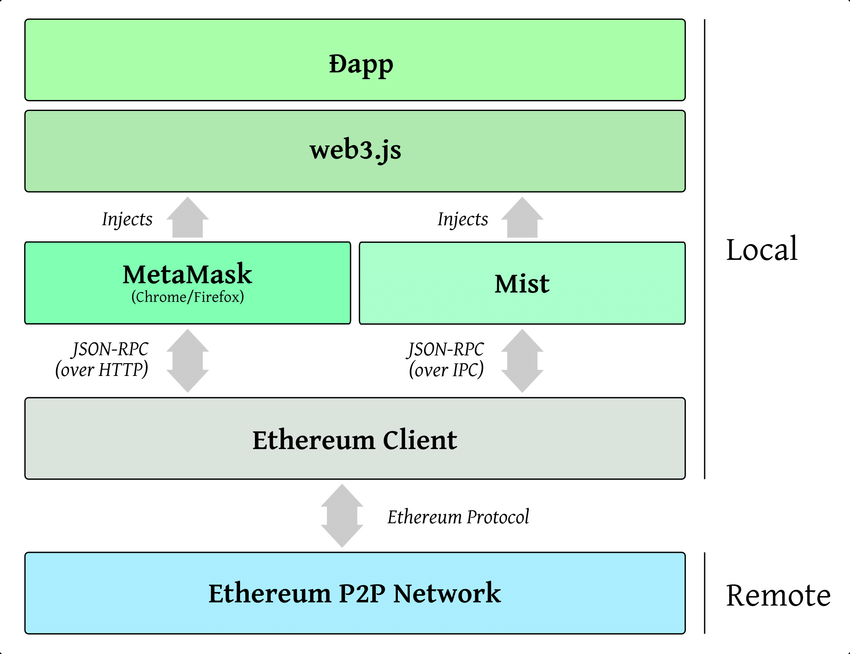
\includegraphics[scale=0.4]{dapp-architecture}
\caption{Arhitektura decentralizirane aplikacije}
\label{fig:dapp}
\end{figure}

\section{Crypto Roulette}

Crypto Roulette je decentralizirana aplikacija koja implementira kockarsku igru ruleta. Pametni ugovor se nalazi na testentu Ropsten (Ethereum testna mreža, tako da ne trebaju stvari novci za pristup i korištenje aplikacije). frontend dio aplikacije je izgrađen u frameworku zvanom React js. U nastavku slijedi par podataka o aplikaciji, a kasnije na slici \ref{fig:crypto} je korisničko sučelje same aplikacije. 

\begin{itemize}
    \item aplikacija: \url{https://masterthesisv2.firebaseapp.com/}
    \item pametni ugovor: \url{https://bit.ly/2m6bZko}
    \item kod cijele aplikacije: \url{https://github.com/senaa12/PmfSmartContracts/tree/master/app}
\end{itemize}

\begin{figure}[H]
\centering
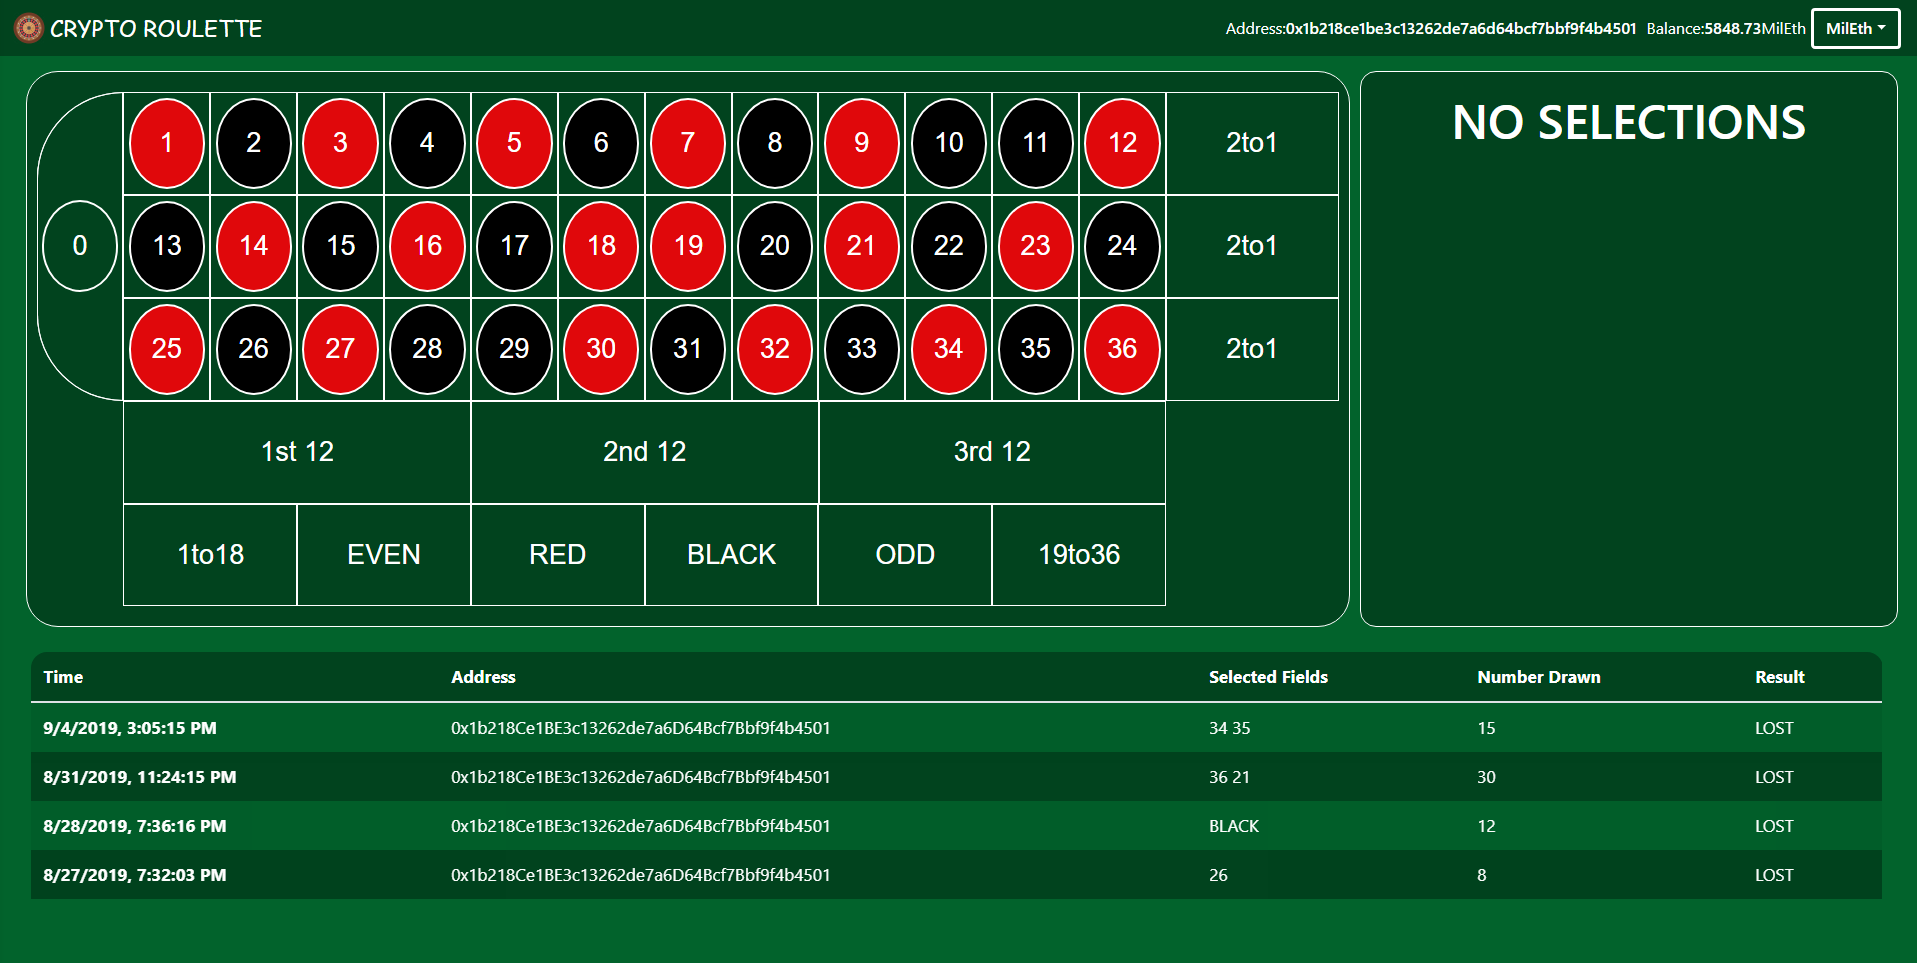
\includegraphics[scale=0.3]{screenshot}
\caption{Crypto Roulette interface}
\label{fig:crypto}
\end{figure}

Decentralizirane aplikacije igara na sreću iako jako popularne trenutno (prema stranici \href{https://www.stateofthedapps.com/}{State Of The DApps} one čine ukupno 18\% svih aplikacija) vrlo su neprirodne u Ethereum okruženju upravo zbog toga što uključuju faktor sreće. U prethodnim poglavljima smo rekli da svaki čvor na mreži za sebe treba potvrditi svaki blok u blockchainu, dakle sve je determinističko. Generacija slučajnih brojeva je u Ethereumu zapravo nemoguća. Prave decentralizirane aplikacije koriste vanjske izvore za generaciju brojeva, s obzirom da Crypto Roulette demonstrativna aplikacija koja služi porebama ovoga rada i jedino je na testnoj mreži, dovoljna je i pseudo random generacija korištenjem hash funkcije sa kombinacijom ovih vrijednosti: vrijeme u kojem je trenutni blok potvrđen, hash-vrijednost prethodnog bloka i prethodno izabrani broj. Hash vrijednost prethodnog bloka i prethodno izabrani broj svi znaju u trenutku klađenja, ali na prvu se čini da je vrijeme potvrđivanja bloka nasumično i to je istina, no čvor koji stvara trenutni blok može kontrolirati vrijeme kada će blok biti potvrđen i samim time on može kontrolirati ishod oklade.

\begin{lstlisting}[caption=Crypto Roulette funkcija koja imitira generaciju brojeva pomoću hash funkcije keccak256 (SHA256) i nije sigurna za stvarnu upotrebu.]
function wheelSpin() public returns (uint) {
        uint _randomNumber = (uint(keccak256(abi.encodePacked(blockhash(block.number - 1), block.timestamp, _lastSpinResults.length)))) % 36;
        _lastSpinResults.push(_randomNumber);
        return _randomNumber;
    }
\end{lstlisting}

Iduća posebnost programiranja pametnih ugovora su \textbf{eventi}. Funkcije koje mjenjaju stanje blockchaina pozivaju se transakcijama, za njih ne znamo unaprijed kada će biti procesirane (naravno možemo otprilike kontrolirati vrijeme podešavanjem cijene gasa, ali ne možemo odabrati točan trenutak). Dakle takve funkcije se ne izvršavaju odmah nego u trenutku kada je blok sa transakcijom koja poziva takvu funkciju potvrđen, zbog toga takve funkcije ne mogu imati nikakvu povratnu vrijednost. Umjesto toga pametni ugovori su uveli evente. Eventi su zapravo spremanje unaprijed definiranih objekata u log transakcija. Event u slučaju Crypto Roullete aplikacije je rezultat jedne oklade, u isječku koda \ref{code:bet} se prikazuje prvo računanje ishoda jedne oklade i na kraju odašiljanje eventa sa rezultatom.

\begin{lstlisting}[caption=Funkcija koja se pokreće prilikom slanja transakcije koja sadrži podatke za igru jedne runde ruleta. Argumenti funkcije su polje \lstinline{betIDs} sa okladama i polje \lstinline{bets} sa iznosima za okladu. Na početku vidimo generaciju broja i računanje dobitka. Tada pametni ugovor\, ako ima dobitka\, u liniji \lstinline{msg.sender.transfer(payoutAmount)} prebacuje dobitnu količinu ethera na adresu igrača. Sve prethodne oklade se čuvaju u polju (primjetimo da je to loš način zapravo\, jer nakon nekog vremena polje će zauzimati mnogo memorije\, pa će i cijena oklade biti skuplja.) U zadnjoj liniji se odašilje event koji se prikazuje na ekranu kao na slici \ref{fig:result}, label={code:bet}]
    function placeBet(uint[] memory betIDs, uint[] memory bets) public payable {
        uint selectedNumber = wheelSpin();
        uint payoutAmount = calculatePayout(selectedNumber, betIDs, bets);
        if(payoutAmount != 0) {
            msg.sender.transfer(payoutAmount);
        }
        Spin memory newSpin = Spin({
            time: block.timestamp,
            better: msg.sender,
            selectedItemID: betIDs,
            totalFundsPlaced: sumArray(bets),
            selectedNumber: selectedNumber,
            isWinningSpin: payoutAmount != 0
        });
        _lastSpins.push(newSpin);
        emit SpinResultEvent(msg.sender, payoutAmount != 0, payoutAmount);
    }
\end{lstlisting}

\begin{figure}[H]
\centering
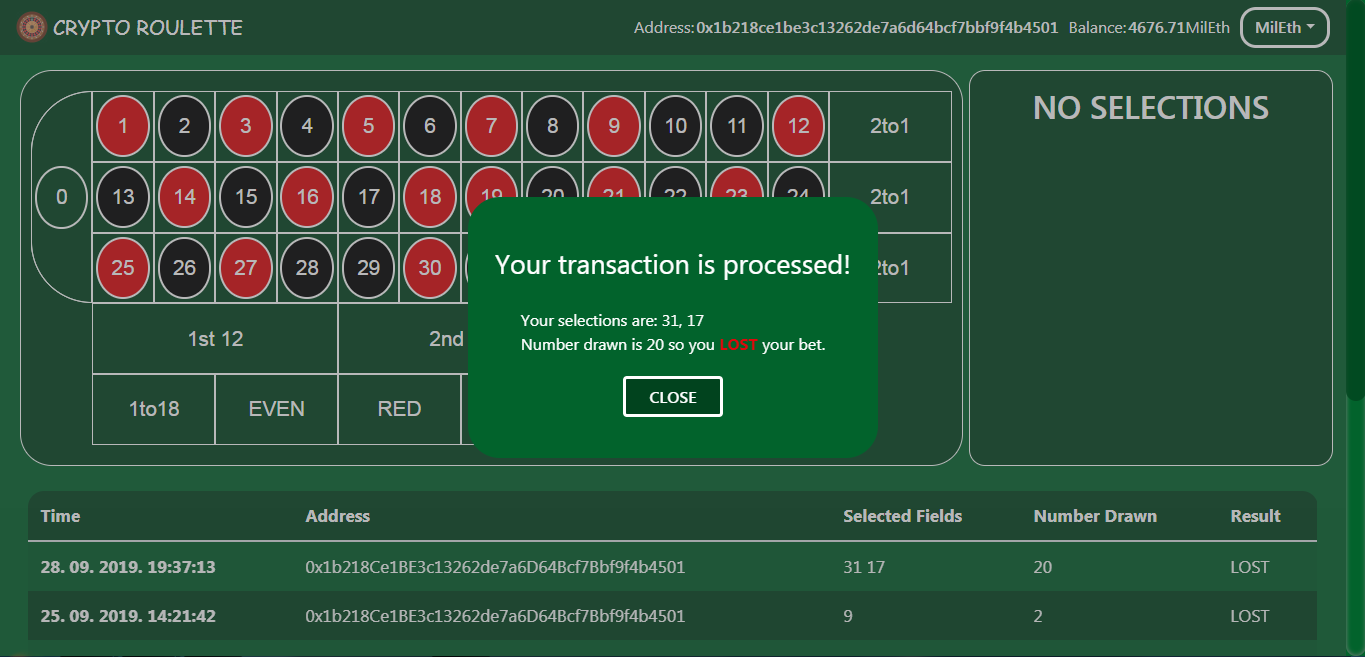
\includegraphics[scale=0.3]{result}
\caption{Crypto Roulette prikaz eventa}
\label{fig:result}
\end{figure}

U prethodnom isječku koda vidimo da pametni ugovor šalje ether jedino u dobitnoj okladi, što je potpuno očekivano. Ether koji je uložen u okladu koja nije dobitna ostaje u pametnom ugovoru i valjalo bi ugraditi mehanizam da se sredstva u ugovoru podignu. No logično je ograničiti podizanje sredstava samo na vlasnika pametnog ugovora ili neku manju skupinu korisnika jer u protivnom igra nema smisla. Upravo u takvom slučaju nam vrlo korisni dolaze \textbf{modifikatori funkcija}. Modifikatori su djelovi koda koji se izvršavaju prije same funkcije i idealni su za provjeravanje raznih uvjeta nad pozvanom funkcijom. Dakle mi želimo provjeriti da li je poziv funkcije za isplatu sredstava došao od vlasnika pametnog ugovora i za to ćemo iskoristiti modifikator funkcije koji se nalazi na idućem isječku koda.

%\begin{minipage}{\linewidth}
\begin{lstlisting}[caption=Ključna riječ \lstinline{modifier} označuje da slijedi modifikator funkcije. U \lstinline{require} naredbu možemo ubaciti sve uvjete koji želimo da budu zadovoljeni\, no tu samo zahtjevamo da je pozivatelj funkcije \lstinline{msg.sender} ujedno i vlasnik pametnog \lstinline{_contractOwner} (lokalna varijabla koja se postavlja u kontruktoru; nema jednostavnog načina za naći vlasnika pametnog ugovora osim ići kroz prošlost transakcija koje uključuju ugovor\, tako da je ovo mnogo jednostavnije i brže.) \\Funkcija payout uplaćuje ether sa ugovora \lstinline{address(this).balance} pozivatelja funkcije (tj. vlasnika ugovora), label={code:modif}, hspace={0.5cm}]
modifier onlyOwner() {
    require(
        msg.sender == _contractOwner,
        "Only Owner can call this function"
    );
    _;
}
    
function payout() public onlyOwner payable {
    return msg.sender.transfer(address(this).balance);
}
\end{lstlisting}
%\end{minipage}

Za kraj još samo napomenimo ovo: Svi isječci kodova, primjeri bytecodova i sl. koji se nalaze u ovome radu su djelovi našeg Crypto Roulette pametnog ugovora.

\chapter{Zaključak}

Prema stranici State Of The DApps koja prati stanje decentraliziranih aplikacija ne samo na Ethereumu već i na ostalim blockchainima dnevno se napravi 1,7 milijun transakcija na decentraliziranim aplikacijama sa prometom od 15 milijuna dolara. Te brojke pokazuju da blockchain i decentralizirane aplikacije su u konstantnom porastu i razvoju što vidimo i na slici \ref{fig:stats} (valja napomenuti da je to statistika samo aplikacija koje se nalaze na stranici StateOfDapps, dakle aplikacija mora biti registrirana tamo, tako da je stvarni broj vjerojatno i veći). Čak za vrijeme pisanja ovoga rada Metamask je izdao alpha verziju mobilnog ethereum preglednika (koji je ujedno i wallet s kojim se direktno mogu slati transakcije) i time postao prvi mobilni preglednik s kojim se može pristupiti decentraliziranim aplikacijama što je veliki korak s obzirom na činjenicu da u današnje vrijeme sve se nalazi na mobitelu.

\begin{figure}[H]
\centering
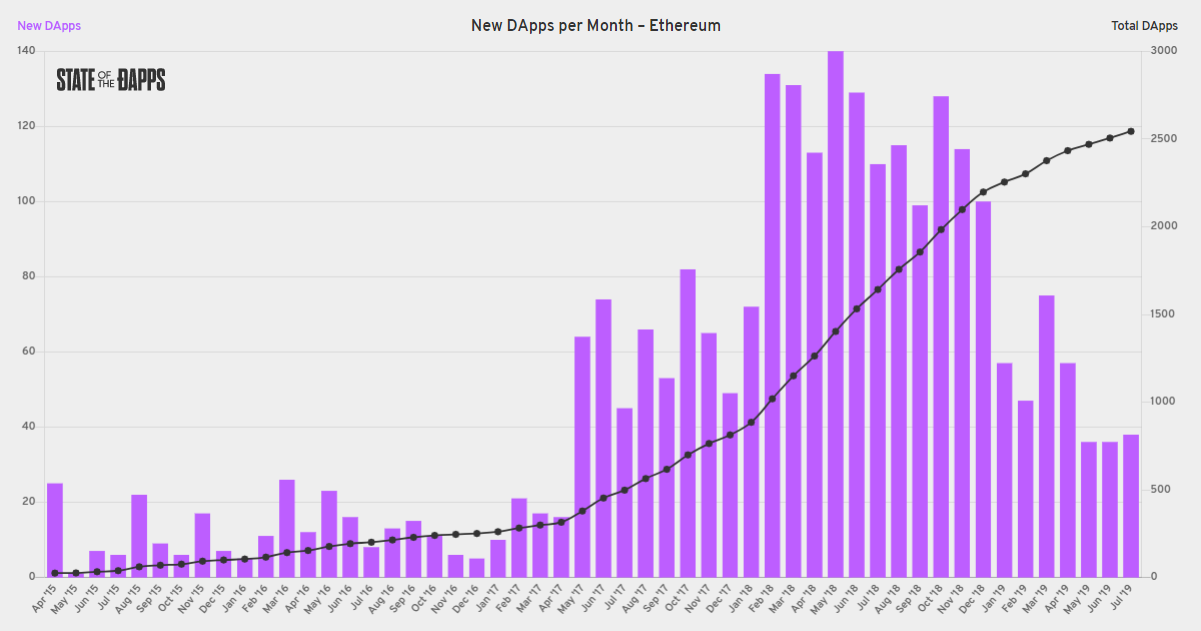
\includegraphics[scale=0.37]{dapps_stats}
\caption{Broj decentraliziranih aplikacija}
\label{fig:stats}
\end{figure}

\newpage

Čak i u fizičkom svijetu oko nas vidimo sve više primjera lokalnih dućana koji prihvaćaju Bitcoin kao način plaćanja. Naime trenutno nema nikakve regulative oporezivanja kriptovaluta i s obzirom na naučeno kroz ovaj rad možemo zaključiti da će to biti jako teško ostvarivo. Iako je Venezuela u ožujku 2018. izdala službenu državnu kriptovalutu Petro s kojom je dopušteno plaćanje u cijeloj državi. Kao primjer korištenja pametnih ugovora imamo Francusku osiguravajuću kuću AXA, koja svoj program osiguranja od kašnjenja letova ima na Ethereumu \cite{axa}.

Primjera postoji sve više iz dana u dan i sve prethodno navedene činjenice nas dovode do istih zaključaka. To jest da i u fizičkom svijetu, kao način plaćanja, ali i u digitalnom svijetu, kao decentralizirane aplikacije, kriptovalute i pametni ugovori imaju svjetlu budućnost.


\bibliography{bibliografija}

\pagestyle{empty} % ne zelimo brojanje sljedecih stranica

% I na koncu idu sazeci na hrvatskom i engleskom

\begin{sazetak}
Kriptovalute zbog svoje vrijednosti trenutno su jedna od popularnijih tema u informatičkom društvu. Većina ljudi ih zamišlja samo kao način plaćanja, no one mogu biti mnogo više od toga i ovaj rad se fokusira na istraživanje kriptovaluta upravo u takvom širem kontekstu. Predstavlja ih kao decentraliziranu mrežu i daje primjere na koji način mogu utjecati na svakodnevni život. Takvu mogućnost nam pružaju pametni ugovori s kojima je moguće napisati proizvoljni računalni program i poslati ga da se izvršava na toj mreži.

Decentralizirana aplikacija je naziv za moderne aplikacije građene pomoću pametnih ugovora. Cilj ovoga rada je potpuna implementacija jedne takve aplikacije i istraživanje teorijske pozadine potrebne za shvaćanje rada iste. Naša decentralizirana aplikacija zove se Crypto Roulette i nalazi se na: \url{https://masterthesisv2.firebaseapp.com/}.

U prvom dijelu rada prvo se iskazuju sva teorijska znanja potreba za shvaćanje decentraliziranih aplikacija. Na početku predstavljamo kriptografske tehnike koje čine bazu svih kriptovaluta da bi nakon toga mogli objasniti Bitcoin, a nakon toga i Ethreum što je mreža na kojoj se izvršavaju pametni ugovori koje ćemo mi proučavati. Nadalje ćemo promotriti same ugovore, njihove mogućnosti, cijene izvršavanja, sigurnost i načine pozivanja koda.

Drugi dio se fokusira na praktičnu primjenu teorije iz prvog dijela pri gradnji decentralizirane aplikacije. Dakle predstavljamo cijelu arhitekturu same aplikacije te navodimo alate koji se koriste pri izgradnji. 

Konačno predstavljamo ukratko samu aplikaciju, analiziramo djelove koda pametnog ugovora Crypto Roulette aplikacije i ističemo razlike od "klasičnog" programiranja aplikacije. U zaključku dajemo primjere iz svakodnevnice gdje se koriste pametni ugovori i naša predviđanja za budućnost.
\end{sazetak}

\begin{summary}
Because of their current value, cryptocurrencies are one of the more popular topics in computer society. To most of the people, they are just the way of paying, but can be so much more and this master thesis focuses on researching cryptocurrencies in that wider context. It presents them as a decentralized network and gives examples in which way they affect everyday life. Smart contracts give us a possibility to write an arbitrary computer program, send it in a transaction and then run it on the network.

A decentralized application is a name for modern application build from smart contracts. A purpose of this thesis is full implementation of one application of that kind and researching theoretic background to understand its working. Our decentralized application is called Crypto Roulette and hosts on: \url{https://masterthesisv2.firebaseapp.com/}.

In the first part of theses initially, we state all theoretical knowledge required to understand the decentralized application. In the beginning, we present cryptography that makes a base for all cryptocurrencies so later we can introduce Bitcoin, and after that Ethereum - which is a network where our smart contracts runs. After that we will observe contracts itself, their possibilities, running prices, security and ways to call code.

The second part focuses on the practical use of theory from the first part when building a decentralized application. Therefore we present the architecture of the entire application while listing tools used in the development process.

Finally, we present an application itself, analyze code of the Crypto Roulette smart contract and emphasize differences between "classical" application development and decentralized one. In the conclusion part, we list examples from every day where smart contracts are used and our predictions for the future.
\end{summary}

% te zivotopis

\begin{cv}
Rođen sam 9. prosinca 1994. godine u Zagrebu. Završio sam Osnovnu školu "Ante Kovačića" i Prirodoslovno-matematičku gimnaziju Lucijana Vranjanina također u Zagrebu. U osnovnoj školi sam sudjelovao na natjecanjima iz matematike i informatike. Bavim se košarkom dugi niz godina i predstavljam fakultet na sveučilišnom prvenstvu. Kao predstavnik Zagrebačkog sveučilišta 2017. sam bio državni prvak u 3x3 košarci.

Nakon završetka srednjoškolskog obrazovanja upisujem preddiplomski sveučilišni studij Matematika na Prirodoslovno-matematičkom fakultetu. Isti završavam 2016. godine postavši tako prvostupnik matematike. U rujnu iste godine upisujem sveučilišni diplomski studij Računarstvo i matematika na istom fakultetu.

U zimskom semestru akademske godine 2017./2018. bio sam na Erasmusu+ programu na Sveučilištu u Ljubljani gdje sam stekao dosta praktičnoga znanja koje mi i danas koristi.

Od srpnja 2018. godine zaposlen sam na poziciji softverskog inženjera u tvrtci Syskit, gdje trenutno radim na razvoju proizvoda Syskit Security Manager koji se koristi za lakšu administraciju Microsoftovog Office365 okruženja.
\end{cv}

\end{document}